\chapter{Static Unit Testing}
The main goal of static unit testing is to find the defects as close as to their point of origin. The review techniques that are applied in the static unit testing are \emph{inspection} and \emph{walkthrough} \autocite{naik2011software}.
\begin{itemize}
    \item \textbf{Inspection:} It is a step-by-step peer group review of a work product, with each step checked against predetermined criteria.
    \item \textbf{Walkthrough:} It is a review where the author leads the team through a manual or simulated execution of the product using predefined scenarios.
\end{itemize}
In this section, only inspection will be considered. A given code will be examined against a checklist by multiple groups of students.

\section{Code Review}
Code quality is a crucial concept for many organizations. Code review is a technique that aims to increase code quality. It can be performed by either an expert or a computer. Nowadays, almost all compilers have a static code analyzer that performs some of the code review tasks. Generally, a checklist is utilized to perform a code review. This checklist can be language-specific or general. A general checklist is given in Table \ref{tab:code-checklist} as an example.

Organizations can develop their own checklists. One important point while doing so is that if a language-specific checklist is produced, then a new checklist should be produced for each language that is used.

After performing an inspection, a report is created which is signed by all participants. The report includes the found defects and problems, the degree of importance of the found problems, and the judgments of participants. The report has three acceptance criteria. They are \emph{accept}, \emph{conditional accept}, and \emph{reinspect}.

\begin{table}[H]
    \centering
    \renewcommand{\arraystretch}{1.2}
    \caption{Code review checklist.}
    \label{tab:code-checklist}
    \begin{adjustbox}{max height=\textheight, max width=\textwidth}
        \begin{tabular}{p{\textwidth}}
            \toprule
            1. Does the code do what has been specified in the design specification?\\
            2. Does the procedure used in the module solve the problem correctly?\\
            3. Does a software module duplicate another existing module which could be reused?\\
            4. If library modules are being used, are the right libraries and the right versions of the libraries being used?\\
            5. Does each module have a single entry point and a single exit point? Multiple exit and entry point programs are harder to test.\\
            6. Is the cyclomatic complexity of the module more than 10? If yes, then it is extremely difficult to adequately test the module.\\
            7. Can each atomic function be reviewed and understood in 10–15 minutes? If not, it is considered to be too complex.\\
            8. Have naming conventions been followed for all identifiers, such as pointers, indices, variables, arrays, and constants? It is important to adhere to coding standards to ease the introduction of a new contributor (programmer) to the development of a system.\\
            9. Has the code been adequately commented upon?\\
            10. Have all the variables and constants been correctly initialized? Have correct types and scopes been checked?\\
            11. Are the global or shared variables, if there are any, carefully controlled?\\
            12. Are there data values hard coded in the program? Rather, these should be declared as variables.\\
            13. Are the pointers being used correctly?\\
            14. Are the dynamically acquired memory blocks deallocated after use?\\
            15. Does the module terminate abnormally? Will the module eventually terminate?\\
            16. Is there a possibility of an infinite loop, a loop that never executes, or a loop with a premature exit?\\
            17. Have all the files been opened for use and closed at termination?\\
            18. Are there computations using variables with inconsistent data types? Is overflow or underflow a possibility?\\
            19. Are error codes and condition messages produced by accessing a common table of messages? Each error code should have a meaning, and all of the meanings should be available at one place in a table rather than scattered all over the program code.\\
            20. Is the code portable? The source code is likely to execute on multiple processor architectures and on different operating systems over its lifetime. It must be implemented in a manner that does not preclude this kind of a variety of execution environments.\\
            21. Is the code efficient? In general, clarity, readability, or correctness should not be sacrificed for efficiency. Code review is intended to detect implementation choices that have adverse effects on system performance.\\
            \bottomrule
        \end{tabular}
    \end{adjustbox}
\end{table}

\section{Exercises}
Given the following problem;
\begin{displayquote}
    Write a function called \lstinline!bool multiple(int, int)! that determines whether the second integer is a multiple of the first for a pair of integers. The function should take two integer arguments and return true if the second is a multiple of the first, otherwise false. Use this function in a program that inputs a series of pair of integers.
\end{displayquote}
a solution is proposed. It might be a correct implementation or not. It is not important for the context of this section.
\begin{lstlisting}[language=C++]
#include <iostream>
using namespace std;

bool multiple(int, int);
int func2(int);

int main() {
    int x, num2;
    bool a;
    cout << "Enter two integers: ";
    cin >> x >> num2;
    a=multiple(x, num2);
    if(a) {
        cout << num2 << " is a multiple of " << x;
    }
    else
        cout << num2 << " is not a multiple of " << x;
}

bool multiple(int X, int num2) {
    if (num2 % X = 0)
        return true;
        else return false;
}

bool func2(int n) {
    int i;
    for(i = 2; i <= n / 2; i++) {
        if(n % i== 0)
            return false;
    }
    return true;
}
\end{lstlisting}
Perform the following exercises.

\begin{exercise}
    Perform a code review to check problems/defect types in this C Program considering the Table \ref{tab:code-checklist}. Write the line number and the type of the problem/defect to the following table.
    
    \begin{table}[H]
    \centering
    \renewcommand{\arraystretch}{1.2}
    \caption{List of found defects.}
    \label{tab:defects-ex}
    \begin{tabular}{p{0.05\textwidth}|p{0.3\textwidth}|p{0.55\textwidth}}
        \toprule
        \# & Line number & Type of the problem/defect\\
        \midrule
        1 & & \\
        \midrule
        2 & & \\
        \midrule
        3 & & \\
        \midrule
        4 & & \\
        \midrule
        5 & & \\
        \midrule
        6 & & \\
        \midrule
        7 & & \\
        \midrule
        8 & & \\
        \midrule
        9 & & \\
        \midrule
        10 & & \\
        \bottomrule
    \end{tabular}
\end{table}
\end{exercise}

\begin{solution}
    No solution has been suggested.
\end{solution}

\begin{exercise}
    Read the following description of the process of the passenger check of a Passenger Service System. Perform a review to check whether all the steps are met in terms of activities in the following activity diagram. Complete the diagram by adding the missing parts.
    
    \begin{displayquote}
        In a Passenger Service System, when a passenger arrives at the airport to check in, (s)he first shows his or her ticket at the check-in counter. The ticket will be checked for its validity. If the ticket is not OK, the passenger will be referred to customer service. If the ticket is OK, the passenger will check his or her luggage. If the luggage has excess weight he or she will pay an additional fee. The luggage will be forwarded to baggage transportation. The passenger receives his or her boarding pass. Note that this activity is between the passenger and the passenger service. Another solution is to make the system visible to show the interaction between the passenger service and the system.
    \end{displayquote}
    
    \begin{figure}[H]
        \centering
        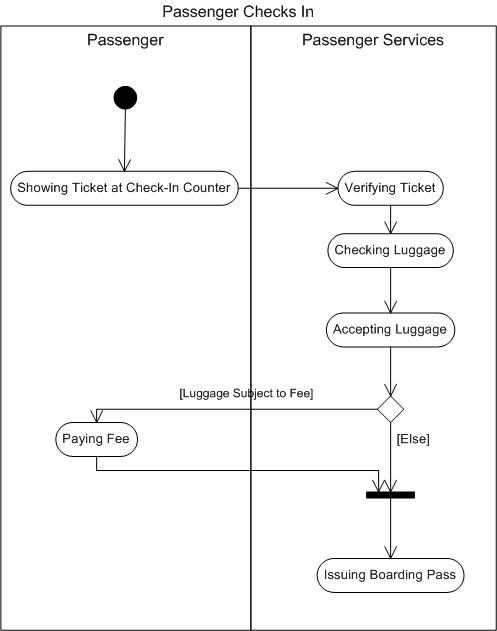
\includegraphics[width=0.8\textwidth]{images/passenger-activity.jpg}
        \caption{Passenger Service System passenger checks in activity diagram.}
        \label{fig:pass-checks-in}
    \end{figure}
\end{exercise}

\begin{solution}
    No solution has been suggested.
\end{solution}
